\documentclass{article}
\usepackage{amsmath, sfmath, multicol, tkz-euclide, array, enumerate, tcolorbox, tabularray}
\renewcommand{\familydefault}{\sfdefault}
\setlength{\parindent}{0cm}
\pagestyle{empty}
\usepackage[left=1in, top=0.5in, right=1in, bottom=0.5in]{geometry}
\tikzset{>=stealth}
\tcbset{colback=white}

\newcounter{example}[section]
\newenvironment{example}[1][]{\refstepcounter{example}\par\medskip
   {\color{red}\textbf{Example~\theexample. #1}}}{\medskip}

\begin{document}

\section*{Slopes of Parallel and Perpendicular Lines}

\begin{tcolorbox}[colframe=orange!70!white, coltitle=black, title=\textbf{Today I Can}]
\begin{enumerate}
    \item Relate slope to parallel and perpendicular lines.
\end{enumerate}
\end{tcolorbox}

\subsection*{Slopes of Parallel Lines}


\begin{itemize}
    \item If 2 non-vertical lines are parallel, then their slopes are equal (and vice versa).
    \item Any 2 vertical lines are parallel.
    \item Any 2 horizontal lines are parallel.
\end{itemize}

\begin{example}
Determine if $a \parallel b$. Justify your answer.

\begin{multicols}{2}
\begin{enumerate}[(a)]
    \item Line $a$: $(-3, \, 3)$ and $(-1, \, -4)$ \newline  Line $b$: $(-1, \, 5)$ and $(2, \, -4)$
    \item Line $a$: $(0, 1)$ and $(5, -2)$ \newline Line $b$: $(0, 4)$ and $(5, 1)$
\end{enumerate}
\end{multicols}
\begin{minipage}{0.5\textwidth}
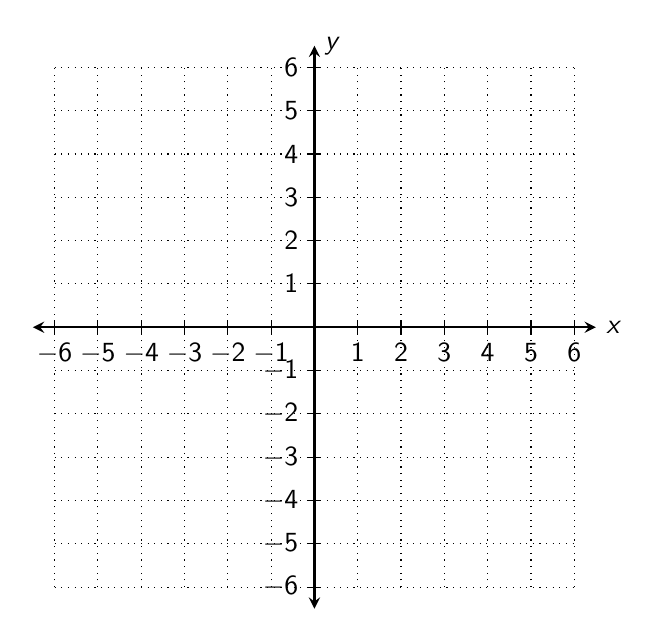
\begin{tikzpicture}[scale=0.55]
    \draw[<->, thick] (-6.5,0) -- (6.5,0) node [right] {$x$};
    \draw[<->, thick] (0,-6.5) -- (0,6.5) node [right] {$y$};
    \draw[dotted] (-6,-6) grid (6,6);
    \foreach \x in {-6,...,-1,,1,...,6}
    \draw (\x, 0.15) -- (\x,-0.15) node [below] {$\tiny \x$};
    \foreach \y in {-6,...,-1,,1,...,6}
    \draw (0.15,\y) -- (-0.15,\y) node [left] {$\tiny \y$};
\end{tikzpicture}
\end{minipage}
\begin{minipage}{0.4\textwidth}
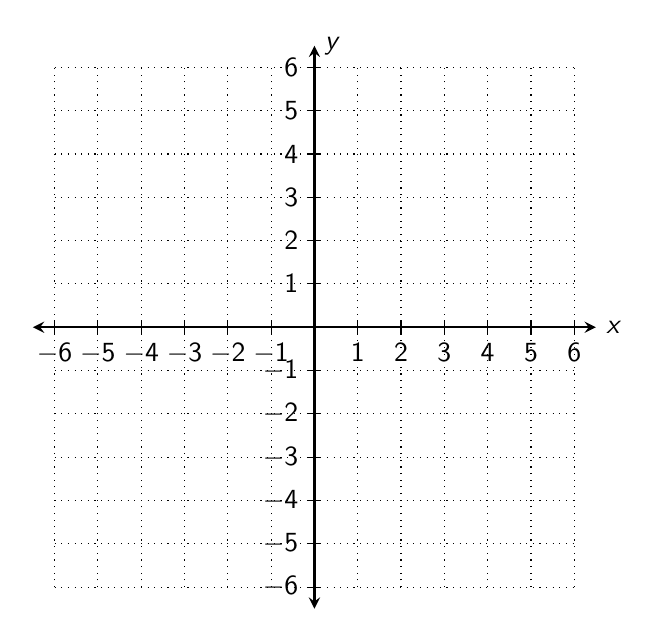
\begin{tikzpicture}[scale=0.55]
    \draw[<->, thick] (-6.5,0) -- (6.5,0) node [right] {$x$};
    \draw[<->, thick] (0,-6.5) -- (0,6.5) node [right] {$y$};
    \draw[dotted] (-6,-6) grid (6,6);
    \foreach \x in {-6,...,-1,,1,...,6}
    \draw (\x, 0.15) -- (\x,-0.15) node [below] {$\tiny \x$};
    \foreach \y in {-6,...,-1,,1,...,6}
    \draw (0.15,\y) -- (-0.15,\y) node [left] {$\tiny \y$};
\end{tikzpicture}
\end{minipage}
\end{example}

\vfill 

\begin{example}
\begin{enumerate}[(a)]
    \item What is the equation of the line parallel to $y=-3x-5$ that contains $(-1, \, 8)$?    \vfill 
    \item What is the equation of the line parallel to $y=-x-7$ that contains $(-5, \, 3)$?     \vfill 
\end{enumerate}
\end{example}

\newpage 

\subsection*{Slopes of Perpendicular Lines}


\begin{itemize}
    \item Opposite signs
    \item Reciprocals
    \item One line is horizontal and the other is vertical
\end{itemize}
\vspace{0.2in}

\begin{example}
Determine whether or not the lines are perpendicular. Justify your answer.

\begin{multicols}{2}
\begin{enumerate}[(a)]
    \item Line $a$: $(-4, \, 2)$ and $(0, \, -4)$ \newline Line $b$: $(-5, \, -3)$ and $(4, \, 3)$
    \item Line $a$: $(1, \, 5)$ and $(-3, \, -3)$ \newline Line $b$: $(4, \, 5)$ and $(-2, \, 2)$
\end{enumerate}
\end{multicols}
\begin{minipage}{0.5\textwidth}
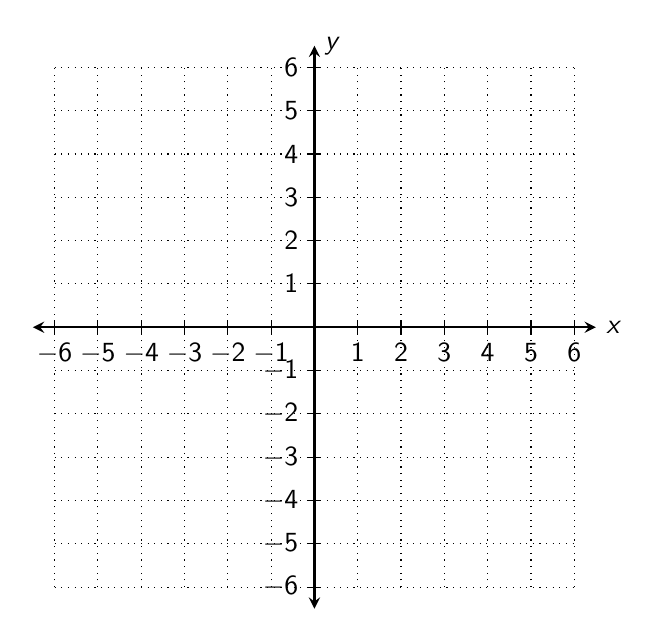
\begin{tikzpicture}[scale=0.55]
    \draw[<->, thick] (-6.5,0) -- (6.5,0) node [right] {$x$};
    \draw[<->, thick] (0,-6.5) -- (0,6.5) node [right] {$y$};
    \draw[dotted] (-6,-6) grid (6,6);
    \foreach \x in {-6,...,-1,,1,...,6}
    \draw (\x, 0.15) -- (\x,-0.15) node [below] {$\tiny \x$};
    \foreach \y in {-6,...,-1,,1,...,6}
    \draw (0.15,\y) -- (-0.15,\y) node [left] {$\tiny \y$};
\end{tikzpicture}
\end{minipage}
\begin{minipage}{0.4\textwidth}
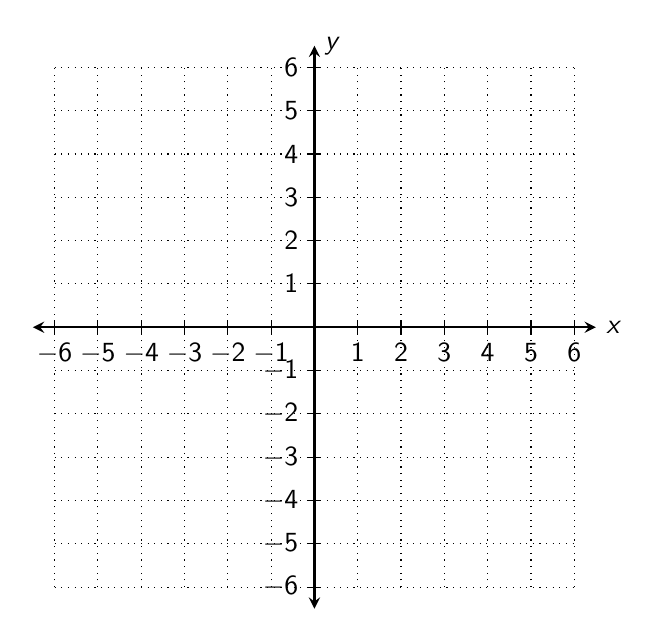
\begin{tikzpicture}[scale=0.55]
    \draw[<->, thick] (-6.5,0) -- (6.5,0) node [right] {$x$};
    \draw[<->, thick] (0,-6.5) -- (0,6.5) node [right] {$y$};
    \draw[dotted] (-6,-6) grid (6,6);
    \foreach \x in {-6,...,-1,,1,...,6}
    \draw (\x, 0.15) -- (\x,-0.15) node [below] {$\tiny \x$};
    \foreach \y in {-6,...,-1,,1,...,6}
    \draw (0.15,\y) -- (-0.15,\y) node [left] {$\tiny \y$};
\end{tikzpicture}
\end{minipage}
\end{example}

\vfill 

\textbf{Example 4.}
\begin{enumerate}[(a)]
    \item What is the equation of the line perpendicular to $y=\frac{1}{5}x+2$ that contains $(15, \, -4)$?     \vfill 
    \item What is the equation of the line perpendicular to $y=-3x-5$ that contains $(-3, \, 7)$?       \vfill 
\end{enumerate}

\end{document}
